\clearpage
\section*{Fetch}
The Fetch stage reads the instructions from the instructions memory and places the arguments into \verb+iCode+, \verb+iFun+, \verb+rA+, \verb+rB+, and \verb+valC+.

\noindent
The \verb+FetchRegEnable+ sub-circuit will allow the Fetch stage to load the value \verb+iCode+, \verb+iFun+, \verb+rA+, and \verb+rB+. The \verb+FetchDataEnable+ sub-circuit will allow the Fetch state to load the value \verb+valC+. Both of these circuits will also handle the varing lengths of instructions and load the appropriate bytes into the output.

\noindent
The \verb+FetchValP+ sub-circuit will allow the Fetch state to load the value \verb+valP+

\noindent
Additionally, when the Fetch stage is done loading the instruction and its required values, a \verb+complete+ pulse is sent. Since the Fetch stage needs to load between one and 10 bytes, the complete flag, using \verb+valP+, will dynamically wait until all the values are loaded.
\subsection*{Contributors}
Huy Lai\\
Arjun Kurkal\\
Kevin Weston

\clearpage
\subsection*{Screenshots}
\begin{figure}[!ht]
    \centering
    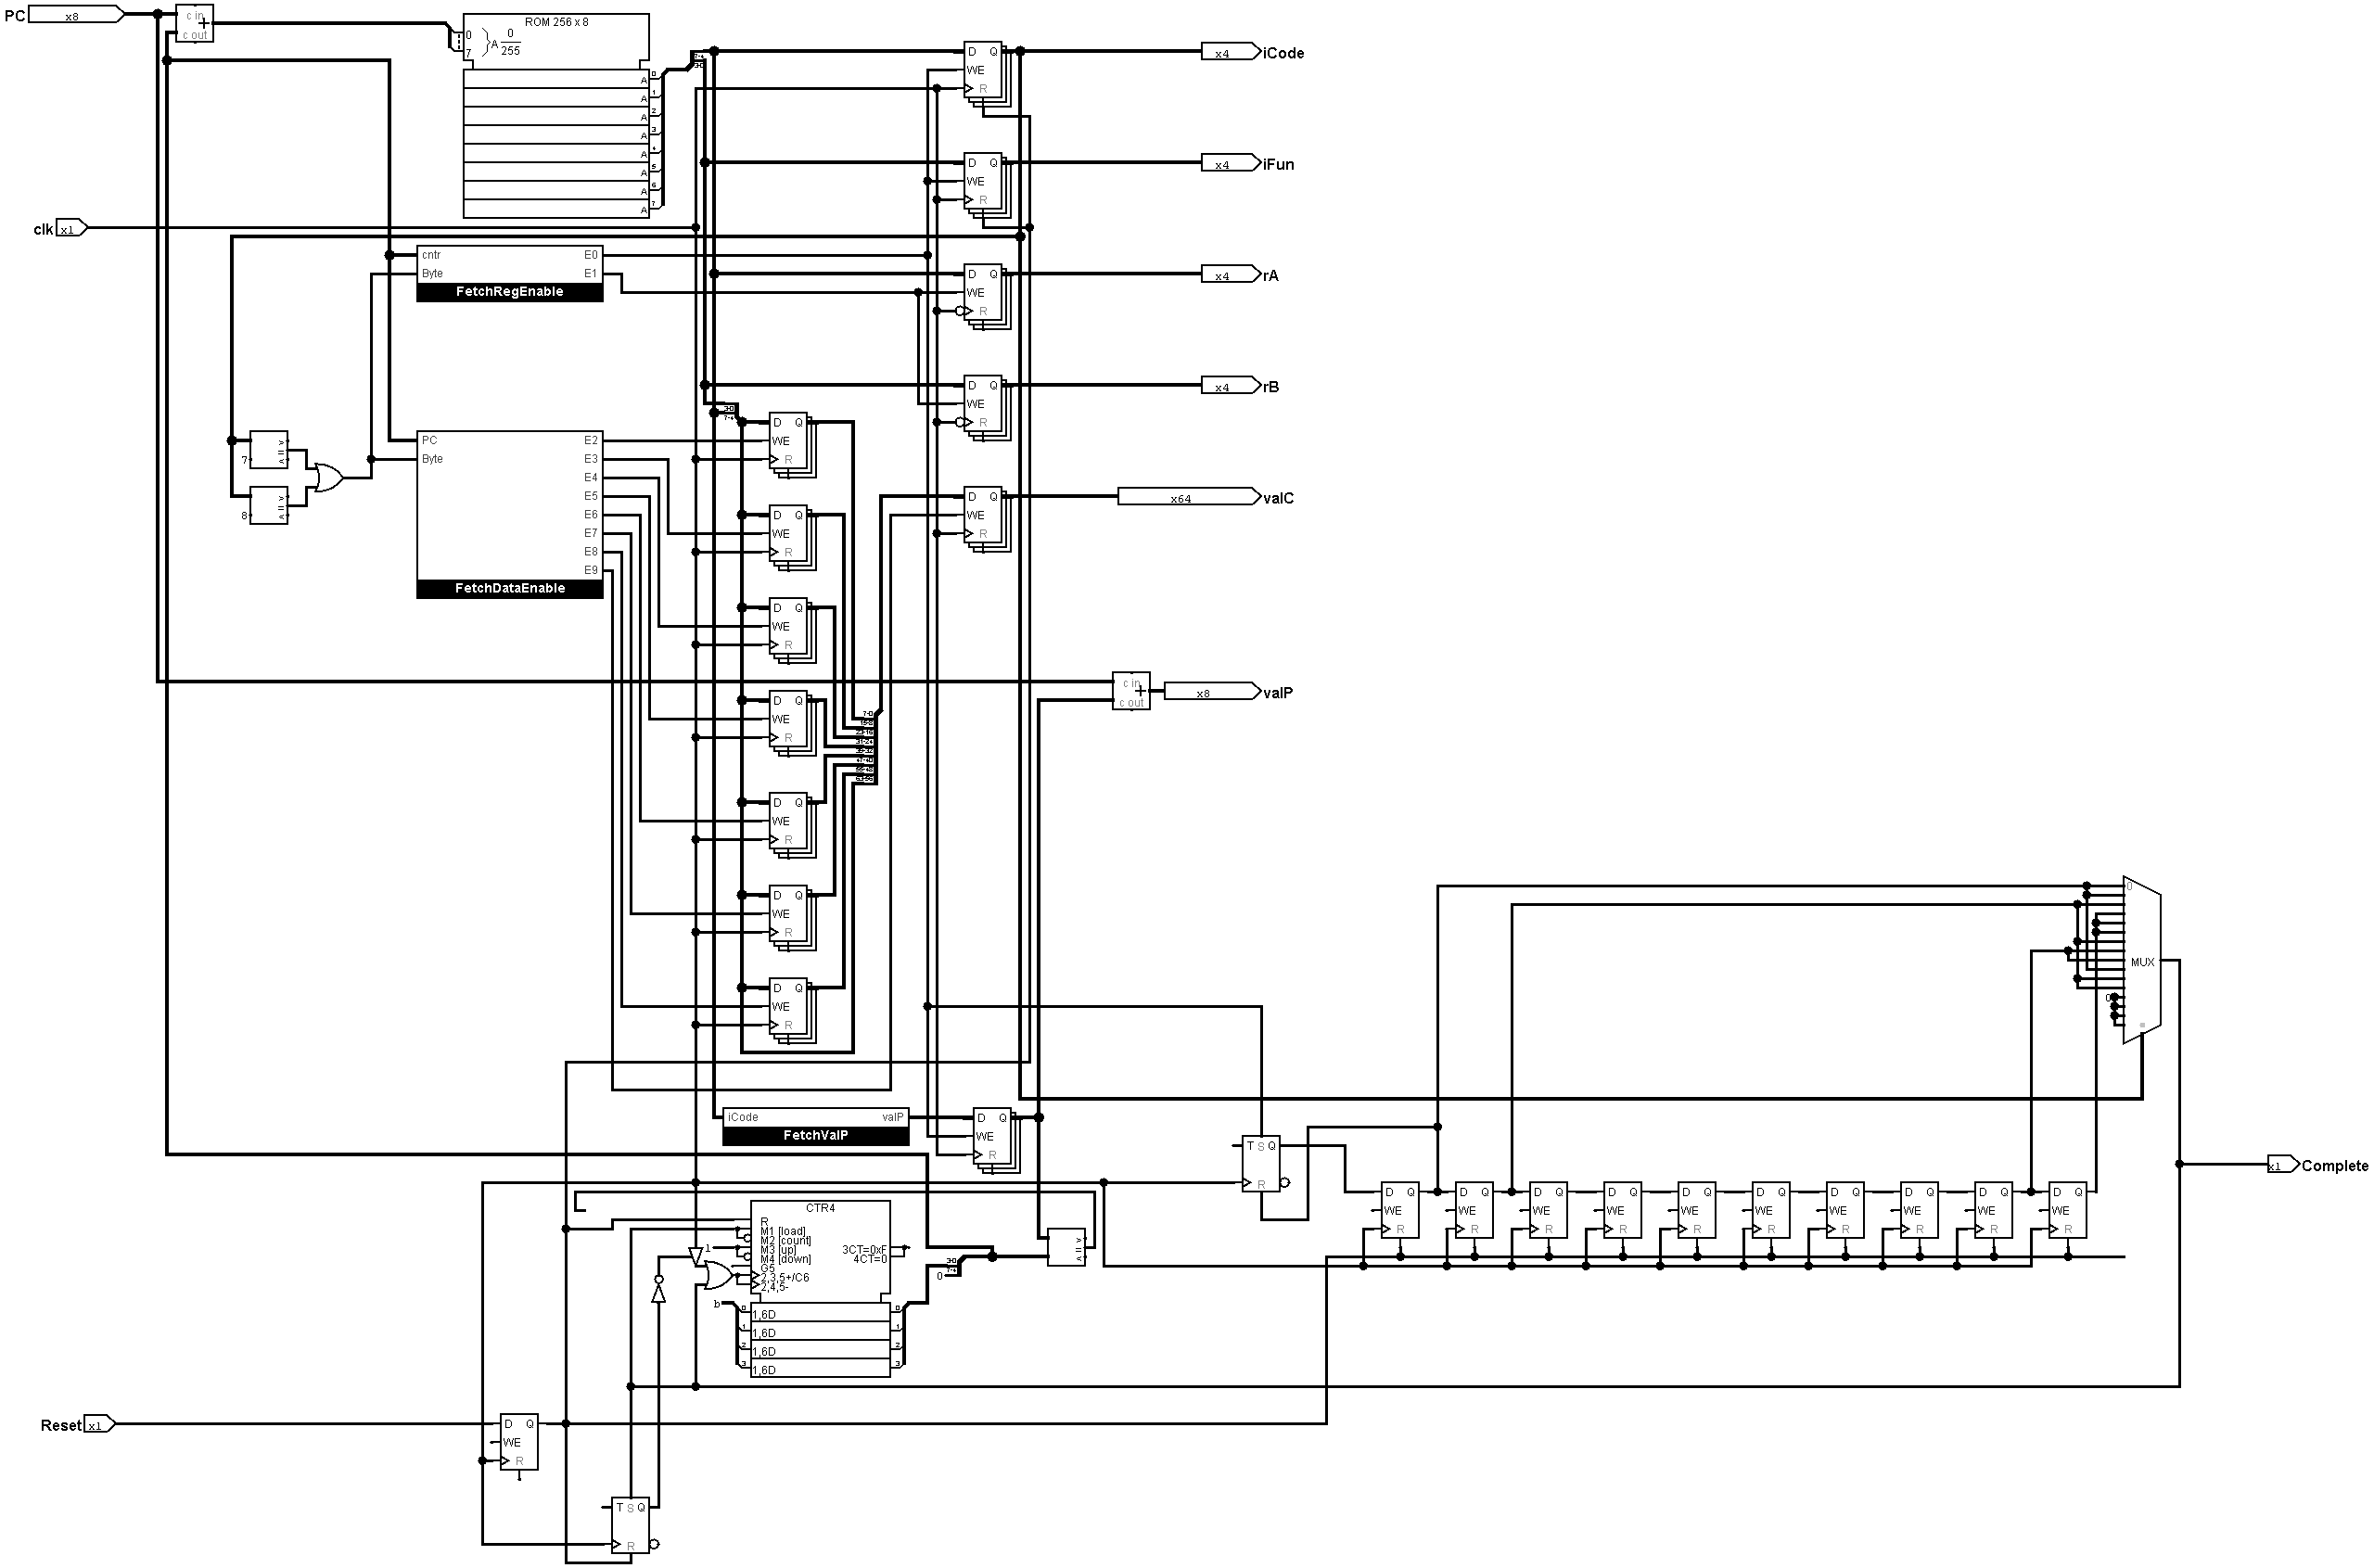
\includegraphics[width=\textwidth]{Images/Fetch.png}
    \caption{Fetch}
\end{figure}

\clearpage
\noindent